\documentclass{report}
\usepackage{graphicx} % Required for inserting images
\usepackage[italian]{babel}
\usepackage{tikz}
\usepackage{hyperref}
\usepackage{amsmath}
\usepackage{xcolor}

\definecolor{darkgreen}{rgb}{0.0, 0.5, 0.0} % RGB per un verde scuro


\title{Privacy e Protezione dei dati in Scenari Emergenti}
\date{Parte I}

\begin{document}

\maketitle

\tableofcontents

\newpage
Una continua crescita riguardante:
\begin{itemize}
    \item database governativi e aziendali
    \item contenuti generati dagli utenti 
    \item informazioni personali identificative collezioante quando un utente crea un account, scarica un'applicazione, \dots
\end{itemize}
La condivisione dei dati serve per:
\begin{itemize}
    \item studiare le tendenze e fare inferenze statistiche
    \item condividere conoscenza
    \item accedere ai servizi online
\end{itemize}
C'è inoltre l'archiviazione e il calcolo esterno (cloud), che offorno:
\begin{itemize}
    \item risparmio sui costi e benefici dei servizi
    \item maggiore disponibilità e protezione da eventuali disastri
\end{itemize}

\textbf{Per questa serie di motivazioni è fondamentale garantire che la privacy e l’integrità dei dati siano
adeguatamente protette.}

\chapter{Privacy nella Pubblicazione dei Dati}

Quando si parla del rilascio di informazioni per scopi statistici,
è possibile fare una distinzione tra:
\begin{itemize}
    \item \textbf{statistical DBMS:} c'è un'interazione tra client e DBMS, con quest'ultimo che risponde a delle query. Richiede un \textbf{controllo a runtime} delle informazioni rilasciate.
    \item \textbf{statistical data:} non c'è un'interazione; il controllo viene fatto prima del rilascio dei dati, tramite delle autorità competenti
\end{itemize}

\section{Macrodata, microdata, disclosure}
Per \textbf{macrodata} si intendono dati aggregati; le tabelle possono essere classificate in due gruppi:
\begin{itemize}
    \item \textbf{Conteggio/Frequenza:} ogni cella contiene il numero o la percentuali di rispondenti che hanno lo stesso valore per gli attributi considerati.
    Mostrano il numero di volte che un valore compare nei dati (quanti studenti hanno preso un certo voto).
    \item \textbf{Magnitudo:} ogni cella contiene un valore di una \textit{quantità di interesse}. 
    Riportano la somma o media di un valore numerico associato a una cateogoria (somma degli stipendi per dipartimento). 
\end{itemize}

Per \textbf{microdata} si intendono dati non aggregati, ovvero dati specifici e individuali; questo 
tipo di dati sono soggetti a un maggiore rischio di violazione della privacy (attacchi di collegamento).

\subsubsection{Rilascio di informazioni}
Il rilascio di informazioni si riferisce all'\textbf{attribuzione di informazioni sensibili a un rispondente}.

Si può fare una distinzione tra:
\begin{itemize}
    \item \textbf{Identity disclosure:} è quando un terzo può \textbf{identificare} un rispondente tramite le informazioni rilasciate; è un problema
    quando si tratta di microdata, dato che i dati sono dettagliati 
    \item \textbf{Attribute disclosure:} è quando \textbf{informazioni confidenziali} di un rispondente sono 
    rilasciate o possono essere a lui attribuite, con esattezza o con un grado di precisione inferiore a quello atteso 
    \item \textbf{Inferential disclosure:} è quando informazioni sensibili vengono \textbf{dedotte con alta certezza dalle proprietà statistiche dei dati rilasciati}.
\end{itemize}

\subsubsection{Tecniche di protezione per macrodata}
\begin{itemize}
    \item \textbf{Sampling:} pubblicare solo una porzione della popolazione totale; deve essere rappresentativo e privo di bias
    \item \textbf{Special rules:} si definiscono delle restrizioni sul livello di dettaglio che può essere fornito (ad esempio, non pubblicare o rendere
    deducibili i redditi sotto un intervallo di 1000\$)
    \item \textbf{Threshold rules:} definire una cella come sensibile se il numero di rispondenti è inferiore a un soglia
\end{itemize}

\subsubsection{Tecniche di protezione per microdata}
\begin{itemize}
    \item \textbf{Masking:} si trasforma il dataset non rilasciando o modificando i suoi valori. Possono essere:
    \begin{itemize}
        \item \textit{non-perturbative:} il dataset non viene modificato, ma alcuni dati sono soppressi o alcuni dettagli rimossi (sampling, generalizzazione)
        \item \textit{perturbative:} il dataset viene modificato (arrotondamento, \\swapping); viene introdotto del rumore
    \end{itemize}
    \item \textbf{Dati sintetici:} vengono usati dati plausibili ma sintetici;
    \begin{itemize}
        \item \textit{fully synthetic:} il dataset contiene solo dati sintetici
        \item \textit{partially synthetic:} il dataset contiene sia dati sintetici che dati originali
    \end{itemize}
\end{itemize}

\newpage
\subsection{Anonimity problem}
È in continua crescita il numero di record che contengono dati sensibili dei cittadini. Questi record
vengono \textit{de-identificati} prima della loro pubblicazione; tuttavia, questo \textbf{non è sufficiente}: possono essere 
usati altri dati per fare dei collegamenti tra identità de-identificate, facendo dunque
una \textbf{re-identificazione}.

\subsubsection{Esempio}
\begin{figure}[ht]
    \centering
    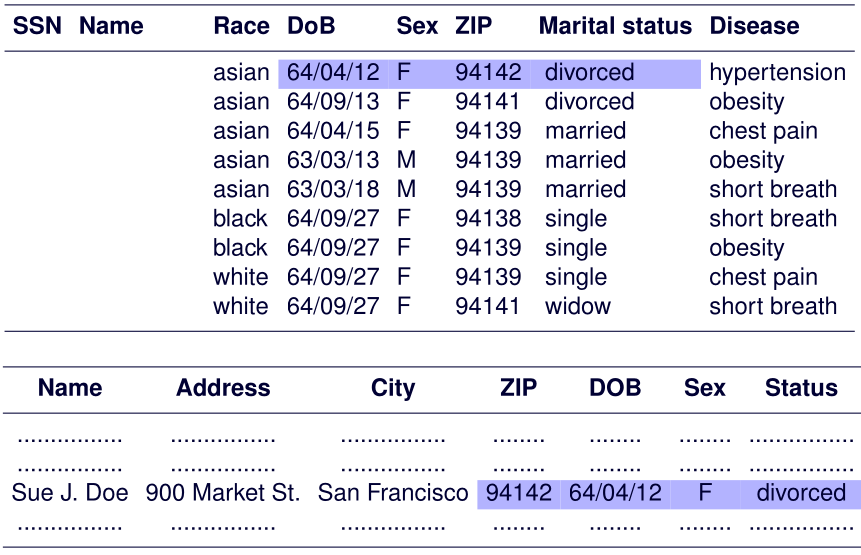
\includegraphics[width=0.9\linewidth]{images/anon-1.png}
\end{figure}
\begin{figure}[ht]
    \centering
    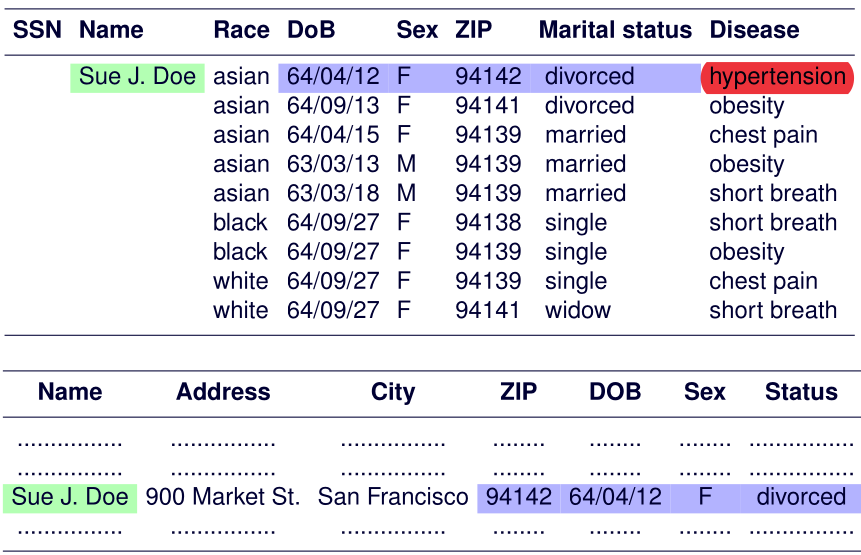
\includegraphics[width=0.9\linewidth]{images/anon-2.png}
\end{figure}

\subsubsection{Classificazione degli attributi in una tabella microdata}

\begin{itemize}
    \item \textbf{Identificatori:} attributi che identificano univocamente un rispondente
    \item \textbf{Quasi identificatori:} attributi che linkati ad informazioni esterne possono reidentificare un rispondente, o ridurre 
    l'incertezza sulla loro identità (Data di nascita, ZIP, sesso)
    \item \textbf{Confidenziale:} attributi sensibili
    \item \textbf{Non confidenziale:} attributi non considerati sensibili
\end{itemize}

\subsubsection{\textcolor{red}{Fattori che contribuiscono al disclosure risk}}
\begin{itemize}
    \item esistenza di record con \textit{caratteristiche peculiari}
    \item possibilità di matchare microdata con informazioni esterne 
\end{itemize}

\subsubsection{\textcolor{darkgreen}{Fattori che diminuiscono il disclosure risk}}
\begin{itemize}
    \item le tabelle spesso contengono un sample della popolazione totale
    \item le tabelle potrebbero non essere aggiornate o esprimere i dati con formati diversi rispetto alle fonti esterne 
    \item le tabelle (anche quelle esterne) contengono rumore
\end{itemize}

\subsubsection{Valutazione del rischio di disclosure}
La valutazione del rischio di \textit{disclosure} viene fatta tenendo in considerazione:
\begin{itemize}
    \item la probabilità che il rispondente di interesse sia presente sulle tabelle di mircodata e sulle tabelle esterne 
    \item la probabilità che le variabili di matching siano registrate in modo linkabile tra microdata e tabella esterna 
    \item la probabilità che il rispondente di interesse è peculiare nella popolazione del file esterno 
\end{itemize}

\newpage
\section{$k$ - anonimity}

La $k$ - anonimity mira a proteggere l'identità dei rispondenti, tramite generalizzazione e soppressione, 
rilasciando allo stesso tempo informazioni veritiere.

Cerca di garantire che \textbf{ogni 
combinazione di quasi identificatori sia correlata indistintamente ad almeno \textit{k} individui}.

\subsubsection{Condizione sufficiente per soddisfare la $k$ - anonimity}
Ogni combinazione di quasi identificatori deve avere almeno $k$ occorrenze.

\subsection{Generalizzazione}
Consiste nel sostituire i valori di un dato attributo con dei valori più generali;
si basa sulla definizione di una \textbf{gerarchia di generalizzazioni}.

\subsubsection{Gerarchia di generalizzazione del dominio}
\begin{itemize}
    \item Una relazione di generalizzazione $\leq_D$ definisce un mapping tra il dominio $D$ e le sue generalizzazioni.
    \item Dati due domini $D_i, D_j \in \text{Dom}$, $D_i \leq_D D_j$ indica che i valori nel dominio $D_j$ sono generalizzazioni dei valori in $D_i$.
    \item $\leq_D$ implica l'esistenza, per ogni dominio $D$, di una gerarchia di generalizzazione del dominio $DGH_D = (\text{Dom}, \leq_D)$:
    \begin{itemize}
        \item $\forall D_i, D_j, D_z \in \text{Dom}: D_i \leq_D D_j, D_i \leq_D D_z \Rightarrow D_j \leq_D D_z \lor D_z \leq_D D_j$. (\textit{relazione d'ordine totale})
        \item Tutti gli elementi massimali di $\text{Dom}$ sono singleton.
    \end{itemize}
    \item Data una tupla di dominio $DT = \langle D_1, \ldots, D_n \rangle$ tale che $D_i \in \text{Dom}$, $i = 1, \ldots, n$, la gerarchia di generalizzazione del dominio di $DT$ è $DGH_{DT} = DGH_{D_1} \times \ldots \times DGH_{D_n}$. 
\end{itemize}  

\newpage
\subsubsection{Esempio}
\begin{figure}[ht]
    \centering
    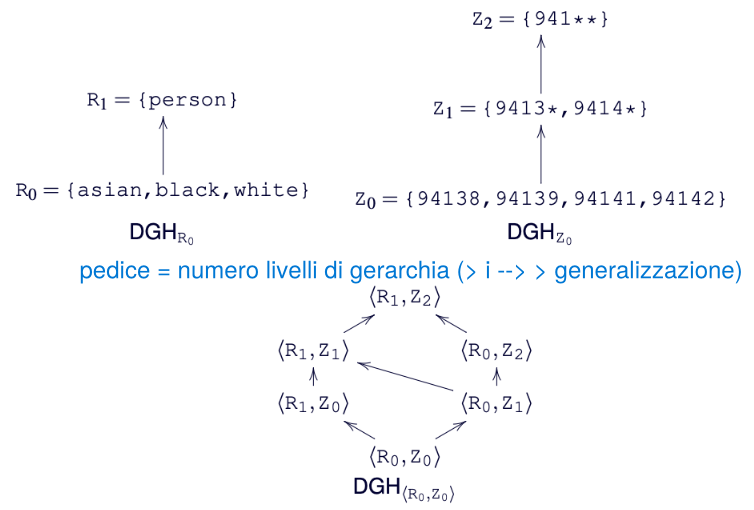
\includegraphics[width=1\linewidth]{images/domger.png}
\end{figure}


\subsubsection{Gerarchia di generalizzazione dei valori}

\begin{itemize}
    \item La relazione di generalizzazione dei valori \( \leq_V \) associa ad ogni valore nel dominio \( D_i \) un valore unico nel dominio \( D_j \), generalizzazione diretta di \( D_i \). 
    \item Questa relazione implica l'esistenza di una gerarchia di generalizzazione dei valori $ VGH_{D} $ per ciascun dominio \( D \).
    \item La $ VGH_{D} $ ha una struttura ad albero:
    \begin{itemize}
        \item \textbf{Foglie}: Rappresentano i valori nel dominio \( D \).
        \item \textbf{Radice}: È il valore più generale, situato nell'elemento massimo di $ DGH_{D} $.
    \end{itemize}
\end{itemize}

\newpage
\subsubsection{Esempio}

\begin{figure}[ht]
    \centering
    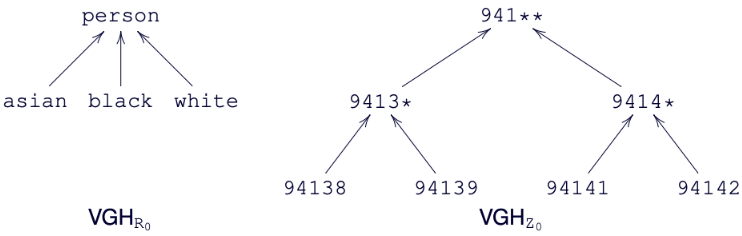
\includegraphics[width=1\linewidth]{images/valuegen.png}
\end{figure}

\subsubsection{Tabella generalizzata con soppressione}
Una tabella \( T_j \) è detta una generalizzazione (mediante soppressione di tuple) della tabella \( T_i \) (\( T_i \preceq T_j \)), se soddisfa le seguenti condizioni:

\begin{itemize}
    \item \( |T_j| \leq |T_i| \)
    \item Il dominio \( \text{dom}(A,T_j) \) di ogni attributo \( A \) in \( T_j \) è uguale o è una generalizzazione del dominio \( \text{dom}(A,T_i) \) dell'attributo \( A \) in \( T_i \).
    \item È possibile definire una funzione iniettiva che associa ogni tupla \( t_j \) in \( T_j \) con una tupla \( t_i \) in \( T_i \), tale che il valore di ogni attributo in \( t_j \) sia uguale o è una generalizzazione del valore dell'attributo corrispondente in \( t_i \).
\end{itemize}

\newpage
\subsubsection{\textit{k-minimal} generalization con soppressione}
Siano \( T_i(A_1, \ldots, A_n) \) e \( T_j(A_1, \ldots, A_n) \) due tabelle tali che \( T_i \preceq T_j \). Il \textbf{vettore di distanza} di \( T_j \) da \( T_i \) è definito come il vettore
\[
DV_{i,j} = [d_1, \ldots, d_n],
\] 
dove ogni \( d_z \) per \( z = 1, \ldots, n \) è la lunghezza del percorso unico tra \( dom(A_z, T_i) \) e \( dom(A_z, T_j) \) nella gerarchia di generalizzazione del dominio \( DGH_{D_z} \).
\\\\\\
Siano \( T_i \) e \( T_j \) due tabelle t.c. \( T_i \preceq T_j \), e sia \( MaxSup \) la soglia specificata di soppressione accettabile. La tabella \( T_j \) è detta una \textbf{generalizzazione k-minimale} della tabella \( T_i \) se e solo se:

\begin{enumerate}
    \item \( T_j \) soddisfa la k-anonymity garantendo la soppressione minima richiesta se per ogni tabella \( T_z \) che soddisfa la k-anonymity e t.c. \( T_i \preceq T_z \) e \( DV_{i,z} = DV_{i,j} \), allora deve valere \( |T_j| \geq |T_z| \).
    \item \( |T_i| \text{ - } |T_j| \leq MaxSup \) (non ho cancellato più del consentito)
    \item \( \forall T_z \text{ t.c. } T_i \preceq T_z \text{ e } T_z \text{ soddisfa le condizioni 1 e 2 } \Rightarrow \neg(DV_{i,z} < DV_{i,j}) \) $ \iff $ \(DV_{i,z} >= DV_{i,j} \)
\end{enumerate}

\subsubsection{Esempio}
$MaxSup = 2$
\begin{figure}[ht]
    \centering
    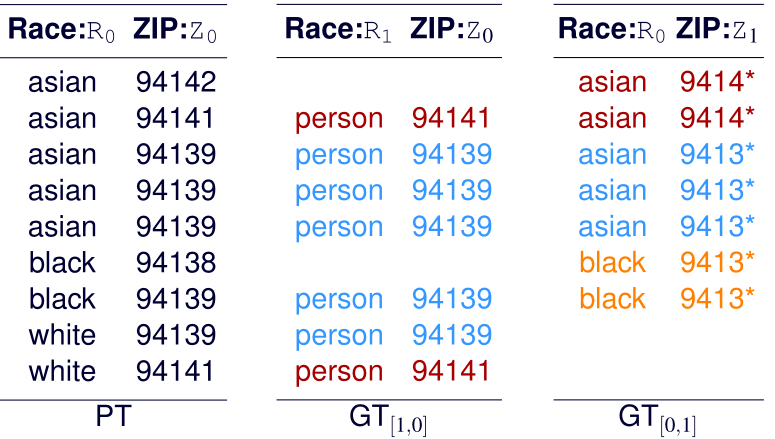
\includegraphics[width=1\linewidth]{images/k-minimal.png}
\end{figure}

\subsection{Computazione di una generalizzazione preferita}
Possono essere applicati diversi criteri di preferenza:
\begin{itemize}
    \item \textbf{Distanza assoluta minima:} minor numeri di passi di generalizzazione
    \item \textbf{Distanza relativa minima:} somma pesata, minimizza il mumero totali di passi relativi
    \item \textbf{Massima distribuzione:} maggior numero di tuple distinte
    \item \textbf{Minima soppressione} 
\end{itemize}

\subsection{Classificazione di tecniche per \textit{k-anonimity}}
Generalizzazione e soppressione possono essere applicate a diversi
livelli di granularità:
\begin{itemize}
    \item \textbf{Generalizzazione:} a livello di colonna o di cella
    \item \textbf{Soppressione:} a livello di riga, di colonna o di cella
\end{itemize}

\newpage
\section{Algoritmi per AG\_TS e AG\_}
\subsubsection{Computing a k-minimal solution}

\begin{itemize}
    \item Ogni percorso in $ DGH_{DT} $ rappresenta una strategia di generalizzazione per \( \text{PT} \)
    \item Chiamiamo \textit{locally minimal generalization} il nodo con indice minore in ogni percorso che soddisfa la \( k \)-anonymity
    \item Proprietà sfruttate dall'algoritmo:
    \begin{enumerate}
        \item Ogni \( k \)-minimal gen è localmente minima rispetto a un percorso, ma il contrario non è vero
        \item Salendo nella gerarchia, il \# di tuple da rimuovere per garantire la \( k \)-anonymity diminuisce
    \end{enumerate}
    \item Se non esiste una soluzione che garantisca la \( k \)-anonymity sopprimendo meno di \( \text{MaxSup} \) tuple all'altezza \( h \), non può esistere una soluzione con altezza inferiore a \( h \) che lo garantisca.
\end{itemize}

\noindent L'algoritmo adotta una ricerca binaria sul reticolo dei vettori distanza:

\begin{enumerate}
    \item Valuta le soluzioni all'altezza \( \left\lfloor \frac{h}{2} \right\rfloor \)
    \item Se esiste almeno una soluzione che soddisfa la \( k \)-anonymity:
    \begin{itemize}
        \item Valuta le soluzioni all'altezza \( \left\lfloor \frac{h}{4} \right\rfloor \)
    \end{itemize}
    \item Altrimenti valuta le soluzioni all'altezza \( \left\lfloor \frac{3h}{4} \right\rfloor \)
    \item Fino a quando l'algoritmo min(h) per la quale esiste un DV che soddisfa la \( k \)-anonymity
\end{enumerate}

\noindent Per ridurre il costo computazionale, l'algoritmo utilizza una matrice di vettori distanza.

\newpage
\subsubsection{k-Optimize algorithm}

\begin{itemize}
    \item Ordinare gli attributi nel quasi-identificatore (\textit{QI}) e i valori nei rispettivi domini.
    \item Associare un indice intero a ciascun valore del dominio, seguendo l'ordine definito.
\end{itemize}

\noindent Ad esempio:
\begin{center}
    \begin{tabular}{cc}
        \textbf{Race} & \textbf{ZIP} \\
        $\langle$[asian: 1] [black: 2] [white: 3]$\rangle$ & $\langle$[94138: 4] [94139: 5] [94141: 6] [94142: 7]$\rangle$ \\
    \end{tabular}
\end{center}

\begin{itemize}
    \item Una generalizzazione è l'unione dei singoli valori di indice.
    \item Il valore più basso in un dominio di attributi viene omesso. Ad esempio, \{6\} corrisponde a:
    \begin{itemize}
        \item \textbf{Race}: \{1\}, cioè: $\langle$[asian or black or white]$\rangle$
        \item \textbf{ZIP}: \{4, 6\}, cioè: $\langle$[94138 or 94139], [94141 or 94142]$\rangle$
    \end{itemize}
    \item L'ordine dei valori all'interno dei domini ha un impatto sulla generalizzazione.
\end{itemize}

\noindent L'algoritmo \textbf{k-Optimize} costruisce un \textbf{albero di enumerazione} per l'insieme degli indici $I$. \\
La radice dell'albero è l'insieme vuoto $\emptyset$, e i figli di ciascun nodo $n$ sono ottenuti aggiungendo un singolo elemento $i$ dell'insieme $I$, tale che $\forall i' \in n, i > i'$. 
Ogni nodo ha un \textbf{costo} che riflette la quantità di generalizzazione e soppressione associata all'anomizzazione rappresentata dal nodo. \\
L'algoritmo cerca l'anonimizzazione con il costo minimo attraverso una \textbf{visita dell'albero} tramite \textbf{ricerca in profondità}. 
Tuttavia, poiché l'albero ha $2^{|I|}$ nodi, la visita completa non è praticabile. Quindi viene adottata una strategia di \textbf{potatura (pruning)}:

\begin{itemize}
    \item Un nodo $n$ viene potato se nessuno dei suoi discendenti può fornire una soluzione ottimale.
    \item Questo si determina calcolando un \textbf{lb:limite inferiore} sul costo dei nodi nel sottoalbero radicato in $n$. 
    Se il limite inferiore è maggiore del miglior costo corrente, il nodo $n$ viene potato.
\end{itemize}

\newpage
\subsubsection{Incognito Algorithm}
L'algoritmo \textbf{Incognito} verifica \textbf{k-anonimity} con riferimento a un adeguato sottoinsieme del QI. \\ 
Esso adotta un approccio \textbf{bottom-up} per visitare le gerarchie di generalizzazione dei domini (DGHs). 
La condizione di k-anonimity rispetto a un sottoinsieme di QI è necessaria, ma non sufficiente per garantire la k-anonimity rispetto a tutto il QI. 
Il processo iterativo dell'algoritmo procede come segue:

\begin{itemize}
    \item \textbf{Iterazione 1}: si controlla la \textbf{k-anonimity} per ciascun attributo singolo in QI, scartando le generalizzazioni che non soddisfano la k-anonimity.
    \item \textbf{Iterazione 2}: si combinano le generalizzazioni rimanenti in coppie, verificando la \textbf{k-anonimity} per ciascuna coppia ottenuta. Scartando le coppie che non soddisfano la k-anonimity.
    \item \textbf{Iterazione n}: si considerano tutte le $n$-uple di attributi ottenuti dalle generalizzazioni che soddisfavano la k-anonimity nell'iterazione $i-1$, scartando le soluzioni che non la rispettano.
    \item $\ldots$
    \item \textbf{Iterazione $|$QI$|$}: restituisce il risultato finale, che rappresenta una generalizzazione che soddisfa la k-anonimity rispetto all'intero quasi-identificatore (QI).
\end{itemize}

\noindent L'algoritmo procede dunque costruendo progressivamente soluzioni, partendo da singoli attributi e combinandoli in gruppi via via più grandi fino a considerare tutti gli attributi del quasi-identificatore.

\newpage
\section{Algoritmi per \_CS e CG\_}

\subsection{Mondrian Multidimensional Algorithm}
L'algoritmo \textbf{Mondrian Multidimensional} si basa su una rappresentazione spaziale delle tuple e dei quasi-identificatori:

\begin{itemize}
    \item Ogni attributo nel quasi-identificatore (\textbf{QI}) rappresenta una dimensione.
    \item Ogni tupla nel set di dati privati (\textbf{PT}) rappresenta un punto nello spazio definito da \textbf{QI}.
    \item Le tuple con lo stesso valore di \textbf{QI} sono rappresentate assegnando una molteplicità ai punti.
    \item Lo spazio multidimensionale viene partizionato dividendo le dimensioni in modo tale che ogni area contenga almeno $k$ occorrenze di valori dei punti. 
    \item Tutti i punti in una regione vengono generalizzati a un valore unico.
    \item Le tuple corrispondenti sono sostituite dalla generalizzazione calcolata.
\end{itemize}

\noindent L'algoritmo Mondrian è flessibile e può operare:
\begin{itemize}
    \item \textbf{Su un numero diverso di attributi:} 
    \begin{itemize}
        \item \textit{Single or Multi-dimension}.
    \end{itemize}
    \item \textbf{Con diverse strategie di generalizzazione:}
    \begin{itemize}
        \item \textit{Global or Local recoding}: colonna o cella.
    \end{itemize}
    \item \textbf{Con diverse strategie di partizionamento:} 
    \begin{itemize}
        \item \textit{Strict or Relaxed partitioning}: senza o con possibili sovrapposizioni.
    \end{itemize}
    \item \textbf{Utilizzando metriche diverse per determinare come dividere ogni dimensione.}
\end{itemize}

\newpage
\subsubsection{Esempio}
Wished $k = 3$
\begin{figure}[ht]
    \centering
    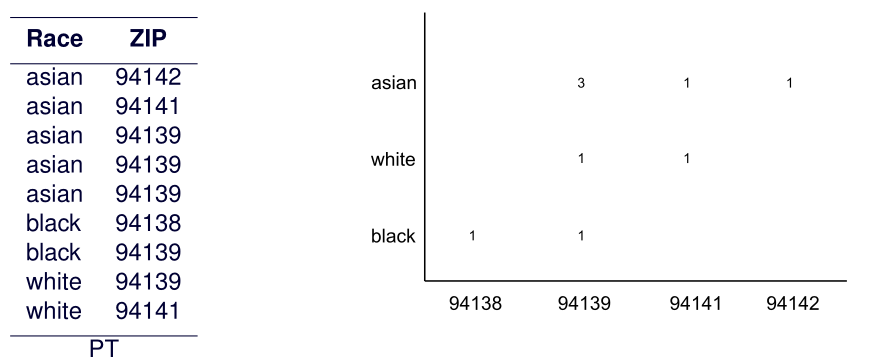
\includegraphics[width=1\linewidth]{images/mondrian1.png}
\end{figure}
\begin{figure}[ht]
    \centering
    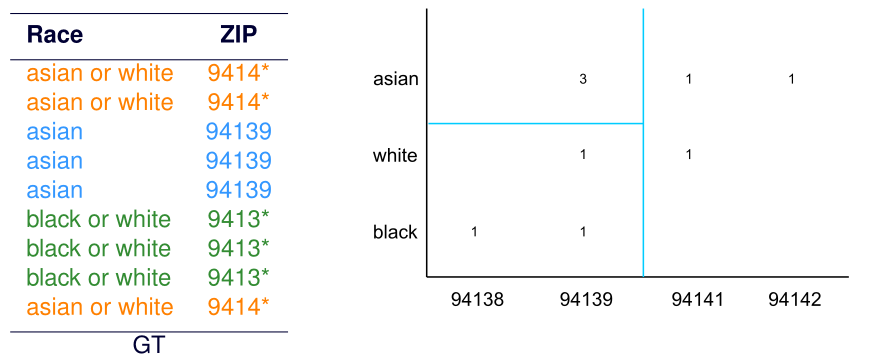
\includegraphics[width=1\linewidth]{images/mondrian2.png}
\end{figure}

\subsection{k-anonymity Revisited}
La \textbf{k-anonymity} cambia a seconda del livello di generalizzazione applicato:

\begin{itemize}
    \item \textbf{AG:} Ogni n-upla di quasi-identificatori deve apparire almeno $k$ volte.
    \item \textbf{CG:} La condizione di avere almeno $k$ occorrenze è sufficiente ma non necessaria. È possibile utilizzare un requisito meno restrittivo:
    \begin{enumerate}
        \item Per ogni sequenza di valori $pt$ in $\mathit{PT[QI]}$, ci devono essere almeno $k$ tuple in $\mathit{GT[QI]}$ che contengono una sequenza di valori che generalizzano $pt$.
        \item Per ogni sequenza di valori $t$ in $\mathit{GT[QI]}$, ci devono essere almeno $k$ tuple in $\mathit{PT[QI]}$ che contengono una sequenza di valori per cui $t$ è una generalizzazione.
    \end{enumerate}
\end{itemize}

\noindent La generalizzazione a livello di cella permette una maggiore flessibilità rispetto alla gen a livello di attributo.








\newpage

\chapter{2}


\subsection{Attribute Disclosure}
La \textbf{k-anonymity} è suscettibile a diversi attacchi:

\begin{itemize}
    \item \textbf{Homogeneity of the Sensitive Attribute Values:} 
    Tutte le tuple con lo stesso QI in una tabella k-anonima possono avere lo stesso valore per l'attributo sensibile.
    \begin{itemize}
        \item Ad esempio, un avversario sa che Carol è una donna di colore e che i suoi dati sono inclusi nella tabella. Se tutte le tuple con quel quasi-identificatore condividono lo stesso valore dell'attributo sensibile, l'avversario può dedurre che Carol soffre di mancanza di respiro.
    \end{itemize}
    
    \item \textbf{Background Knowledge:} 
    Un avversario può utilizzare informazioni esterne già note per dedurre informazioni sensibili.
    \begin{itemize}
        \item Ad esempio, un avversario sa che Hellen è una donna bianca presente nella tabella. Se le opzioni possibili per la sua malattia sono "dolore al petto" o "mancanza di respiro", e l'avversario sa che Hellen corre per 2 ore al giorno, può escludere la "mancanza di respiro" e dedurre che Hellen soffre di "dolore al petto".
    \end{itemize}
\end{itemize}

\subsubsection{\texorpdfstring{$\ell$}{l}-Diversity}
Un \textit{q-block} (cioè, un insieme di tuple con lo stesso valore per i \textit{quasi-identifiers}) è detto $\ell$-diverse se contiene almeno $\ell$ valori differenti e \textit{ben rappresentati} per l'attributo sensibile. 
\begin{itemize}
    \item \textit{ben rappresentati} può essere definito tramite entropia o ricorsione. 
    \item la $\ell$-diversity implica che un avversario deve eliminare almeno $\ell-1$ valori possibili per inferire un valore sensibile di un rispondente.
\end{itemize}

\noindent Una tabella viene definita $\ell$-diverse se tutti i suoi \textit{q-blocks} sono $\ell$-diverse, rendendo impossibili attacchi di omogeneità e più difficili quelli basati su \textit{background knowledge}. 
La $\ell$-diversity è monotona rispetto alle gerarchie di generalizzazione usate per la \textit{k-anonymity}. 
Tuttavia, la $\ell$-diversity può lasciare spazio a nuovi attacchi basati sulla distribuzione dei valori all'interno dei \textit{q-blocks}, come:

\subsubsection{Skewness Attack}
Un \textit{skewness attack} avviene quando la distribuzione dei valori in un \textit{q-block} è diversa da quella della popolazione originale.

\subsubsection{Similarity Attack}
Un \textit{similarity attack} si verifica quando un \textit{q-block} contiene valori diversi ma semanticamente simili per l'attributo sensibile.

\subsubsection{Group Closeness}
Un \textit{q-block} rispetta la \textit{t-closeness} se la distanza tra la distribuzione dei valori dell'attributo sensibile nel \textit{q-block} e nella popolazione è inferiore a una soglia $t$.
\begin{itemize}
    \item Una tabella rispetta la \textit{t-closeness} se tutti i suoi \textit{q-blocks} rispettano tale condizione.
    \item La \textit{t-closeness} è monotona rispetto alle gerarchie di generalizzazione per la \textit{k-anonymity}.
\end{itemize}

\noindent Qualsiasi algoritmo per la \textit{k-anonymity} può essere esteso per rispettare la \textit{t-closeness}, ma tale proprietà può essere difficile da ottenere. 
Inoltre, un osservatore potrebbe usare conoscenze esterne o pregresse per inferire informazioni.

\subsubsection{Types of Background Knowledge}
Le conoscenze possono riguardare:
\begin{itemize}
    \item l'individuo target
    \item altri individui, il che potrebbe comunque rivelare informazioni sensibili
    \item famiglie di valori uguali, come informazioni genomiche che collegano un gruppo di persone.
\end{itemize}

\subsubsection{Multiple Releases}
I dati possono essere soggetti a frequenti cambiamenti e necessitare di pubblicazioni regolari. 
Tuttavia, rilasci multipli di una tabella di microdati possono causare fughe di informazioni poiché un destinatario malevolo può correlare i dataset rilasciati.
 Pertanto, i rilasci multipli (o longitudinali) non possono essere indipendenti, e devono essere protetti contro attacchi di intersezione.

\subsubsection{m-invariance}
Per affrontare il problema dei rilasci longitudinali, una sequenza $T_1, ..., T_n$ di tabelle di microdati rilasciate soddisfa la proprietà di \textit{m-invariance} se:

\begin{itemize}
    \item ogni classe di equivalenza contiene almeno $m$ tuple;
    \item nessun valore sensibile appare più di una volta in ciascuna classe di equivalenza;
    \item per ogni tupla $t$, le classi di equivalenza a cui appartiene $t$ nella sequenza sono caratterizzate dallo stesso insieme di valori sensibili.
\end{itemize}

\noindent Ciò implica che la correlazione delle tuple in $T_1, ..., T_n$ non permette a un destinatario malevolo di associare meno di $m$ valori sensibili differenti a ciascun rispondente.

\subsubsection{Extended Scenarios}
Le tecniche di \textit{k-anonymity}, $\ell$-diversity e \textit{t-closeness} si basano su ipotesi che non sempre sono applicabili in scenari specifici. In particolare:

\begin{itemize}
    \item \textbf{Multiple tuples per respondent}
    \item \textbf{Rilascio di più tabelle con dipendenze funzionali}
    \item \textbf{Più quasi-identificatori}
    \item \textbf{Quasi-identificatori non predefiniti}
    \item \textbf{Rilascio di stream di dati}
    \item \textbf{Preferenze di privacy fine-grained}
\end{itemize}

\subsubsection{ k-anonymity in Various Applications}
Oltre al classico problema del rilascio di microdati, il concetto di \textit{k-anonymity} e le sue estensioni possono essere applicati in diversi scenari, come ad esempio:

\begin{itemize}
    \item \textbf{Social Networks}
    \item \textbf{Data Mining}
    \item \textbf{Location Data}
\end{itemize}

\subsubsection{ Neighborhood Attack in Social Networks}
Un \textit{neighborhood attack} si verifica quando, dato un grafo de-identificato $G'$ di una rete sociale $G$, un avversario sfrutta la conoscenza sui vicini di un utente $u$ per re-identificare il vertice che rappresenta $u$. 

\subsubsection{k-anonymity in Social Networks}
L'idea è di adattare il requisito di \textit{k-anonymity} alle reti sociali. 
Un vertice $u$ è \textit{k-anonymous} se esistono almeno $k-1$ altri vertici $v_1, ..., v_{k-1}$ tali che i sottografi indotti dal vicinato di $u$ e dal vicinato di $v_1, ..., v_{k-1}$ sono isomorfi. 
Un grafo $G'$ è \textit{k-anonymous} se ogni vertice $u$ in $G'$ è \textit{k-anonymous}. 

\noindent \textbf{Intuizione}: aggiungere archi fittizi per soddisfare il requisito di k-anonimato.

\noindent Se $G'$ è \textit{k-anonymous}, con una neighborhood background knowledge, qualsiasi vertice in $G$ non può essere re-identificato in $G'$ con una confidenza maggiore di $1/k$.

\noindent \textbf{Obiettivo}: calcolare una versione \textit{k-anonymous} di una grafo minimizzando il numero di archi aggiunti.

\subsubsection{ k-anonymous Data Mining}
Le tecniche di \textit{privacy-preserving data mining} dipendono dalla definizione di privacy, catturando quali informazioni sono sensibili nei dati originali e dovrebbero essere protette. 
Il \textit{k-anonymous data mining} mira a garantire che i risultati del data mining non violino i requisiti di \textit{k-anonymity} sui dati originali.
Alcuni esempi di tecniche per compromettere la k-anonymity sfruttando il data mining ncludono:

\begin{itemize}
    \item \textbf{Association Rule Mining}: tecniche per trovare regole di associazione possono compromettere la k-anonymity.
    \item \textbf{Classification Mining}: tecniche di classificazione possono portare a minacce per la privacy.
\end{itemize}

\subsubsection{ k-anonymity in Location-Based Services}
Per proteggere l'identità degli utenti in base alla loro posizione geografica, è possibile adottare il concetto di \textit{k-anonymity}, come segue:

\begin{itemize}
    \item Considerare solo le aree che contengono almeno $k$ individui
    \item Ingrandire l'area per includere almeno altri $k-1$ utenti (\textit{k-anonymity})
    \item Obfuscazione delle aree (\textit{location privacy}) per ridurre la precisione o la confidenza dei dati
    \item Protezione del percorso degli utenti (\textit{trajectory privacy}) tramite mix/modifica delle traiettorie
\end{itemize}

\subsubsection{ Re-identification with Any Information}
Qualsiasi tipo di informazione può essere utilizzata per re-identificare dati anonimi. Questo rende la protezione della privacy particolarmente difficile a causa della crescente quantità e varietà di dati raccolti sugli individui. Di seguito, due esempi noti.

\subsubsection{ AOL Data Release}
Nel 2006, AOL pubblicò 20 milioni di query di ricerca effettuate da 650,000 utenti per favorire la comunità di ricerca. Nonostante l'anonimizzazione di username e indirizzi IP, l'uso di numeri identificativi unici permise la re-identificazione di utenti attraverso query specifiche. 
Il caso più noto riguarda \textit{Thelma Arnold}, re-identificata tramite ricerche locali e mediche. Questo evidenzia come dati apparentemente anonimi possano essere utilizzati per risalire all'identità delle persone.

\subsubsection{ Netflix Prize Data Study}
Nel 2006, Netflix lanciò una sfida per migliorare il proprio algoritmo di raccomandazione fornendo un dataset di 100 milioni di record sui rating dei film di circa 500,000 utenti. Studi successivi mostrarono che pochissime informazioni ausiliarie sono necessarie per de-anonimizzare un utente:
\begin{itemize}
    \item Con 6 rating e date (± 2 settimane), il 99\% degli utenti può essere identificato univocamente
    \item Con 2 rating e date (± 3 giorni), il 68\% degli utenti può essere identificato univocamente
\end{itemize}
Informazioni ausiliarie possono essere ottenute da fonti esterne, come IMDb. Questo sollevò preoccupazioni legate alla privacy, poiché le preferenze cinematografiche possono rivelare orientamenti politici, religiosi o sessuali.

\subsubsection{ Other Privacy Breaches}
L'uso di app per il fitness che tracciano la posizione degli utenti ha mostrato come mappe dettagliate possano esporre informazioni sensibili sulla posizione e sull'identità delle persone.

\subsubsection{ Syntactic vs Semantic Privacy Definitions}
\begin{itemize}
    \item \textbf{Syntactic Privacy Definitions}
    Le definizioni di privacy sintattiche misurano il grado di protezione di una persona nei dati con un valore numerico. Ad esempio:
    \begin{itemize}
        \item Ogni rilascio di dati deve essere indistinguibilmente associato ad almeno un certo numero di individui nella popolazione.
    \end{itemize}

    \item \textbf{Semantic Privacy Definitions}
    Le definizioni di privacy semantiche soddisfano un requisito di privacy semantico. Ad esempio:
    \begin{itemize}
        \item Il risultato di un'analisi eseguita su un dataset rilasciato non deve essere influenzato dalla presenza o assenza di una singola tupla nel dataset.
    \end{itemize}
\end{itemize}

\subsubsection{ Differential Privacy}
\begin{itemize}
    \item \textbf{Informal Definition}
    La \textit{differential privacy} mira a prevenire che un avversario sia in grado di rilevare la presenza o assenza di un individuo in un dataset. 
    Ad esempio, il conteggio degli individui affetti da una malattia in un database medico, con un meccanismo che fornisce probabilmente lo stesso risultato su dataset che differiscono per un solo individuo.
    \item \textbf{Formal Definition}
    Una funzione randomizzata $K$ fornisce $\varepsilon$-differential privacy se per tutti i dataset $D$ e $D'$ che differiscono per al massimo una riga, e per ogni insieme $S \subseteq \text{Range}(K)$:
    \[
    \text{Pr}[K(D) \in S] \leq e^{\varepsilon} \times \text{Pr}[K(D') \in S]
    \]
\end{itemize}


\subsubsection{ Differential Privacy Scenarios}
La differential privacy si applica a due scenari principali:
\begin{itemize}
    \item \textbf{Scenario Interattivo}: valutazione di query in tempo reale (Statistical DBMS).
    \item \textbf{Scenario non Interattivo}: rilascio di tabelle di macro-dati pre-calcolate (Statistical Data).
\end{itemize}
Essa viene solitamente implementata tramite l'aggiunta di rumore casuale, ma ciò non preserva necessariamente la veridicità dei dati.

\subsubsection{ Differential Privacy Variations}
Per ridurre la quantità di rumore aggiunto, sono state proposte diverse varianti:
\begin{itemize}
    \item \textbf{($\epsilon$, $\delta$)-differential privacy}: l'approssimazione $\epsilon$ può essere violata con bassa probabilità (controllata da $\delta$).
    \item Metodi basati su trasformate wavelet per migliorare l'utilità dei dati.
\end{itemize}

\subsubsection{ Differential Privacy Applications}
Meccanismi basati su differential privacy sono stati sviluppati per vari domini:
\begin{itemize}
    \item \textbf{Social networks} 
    \item \textbf{Data mining} 
    \item \textbf{Location data}
\end{itemize}

\subsubsection{ Is Differential Privacy Enough?}
La differential privacy limita l'inferenza sulla presenza di una tupla, ma non necessariamente l'inferenza sulla partecipazione di un individuo al processo di generazione dei dati. 
Ad esempio, la partecipazione di Bob in un social network potrebbe influenzare le relazioni tra i suoi amici, non solo la sua tupla.

\subsubsection{ k-anonymity vs Differential Privacy}

\begin{itemize}
    \item \textbf{k-anonymity}:
    \begin{itemize}
        \item \textbf{Pro}: Cattura bene i requisiti del mondo reale.
        \item \textbf{Contro}: Non offre una protezione completa.
    \end{itemize}
    
    \item \textbf{Differential Privacy}:
    \begin{itemize}
        \item \textbf{Pro}: Offre garanzie di protezione migliori.
        \item \textbf{Contro}: Non facile da capire o applicare, e non garantisce una protezione completa.
    \end{itemize}
\end{itemize}


\section{Some Examples of Other Privacy Issues}

\subsection{Sensitive Value Distributions}
\begin{itemize}
    \item Le tuple individuali non sono intrinsecamente sensibili.
    \item Una raccolta di tuple potrebbe rivelare informazioni sensibili non esplicitamente riportate, in particolare a causa di distribuzioni di valori peculiari.
\end{itemize}

\subsubsection{Example: Soldiers' Medical Records}
\begin{itemize}
    \item I record individuali non sono sensibili.
    \item La distribuzione dell'età dei soldati in una località può indicare il tipo di località:
    \begin{itemize}
        \item Soldati giovani suggeriscono tipicamente un campo di addestramento.
        \item Funzionari più anziani indicano un quartier generale.
    \end{itemize}
\end{itemize}

\subsubsection{Counteracting Inference Channels}
\begin{itemize}
    \item La valutazione dell'esposizione dei dati rilasciati può essere effettuata attraverso:
    \begin{itemize}
        \item ll calcolo a priori del numero massimo di tuple rispetto alla baseline distribution, inclusi il numero di rilasci per diversi valori di attributi.
        \item La valutazione delle metriche di esposizione sulle tuple richieste.
    \end{itemize}
\end{itemize}

\subsection{Privacy and Genomic Data}
Le informazioni genomiche presentano opportunità in medicina ma sollevano anche diversi problemi di privacy:
\begin{itemize}
    \item Il genoma umano può identificare il suo proprietario.
    \item Contiene info sensibili sulla provenienza etnica, predisposizione a malattie e altri tratti fenotipici.
    \item I dati genomici possono rivelare informazioni sui parenti e sui discendenti sulla base del genoma.
\end{itemize}

\subsubsection{Individuals' Re-identification}
\subsubsection{Example: The 1000 Genomes Project:} Un'iniziativa internazionale avviata nel 2008 per definire un catalogo della variazione genetica umana. 
Durante il progetto, cinque uomini coinvolti sia in questo progetto sia in uno studio su famiglie mormoni nello Utah sono stati ri-identificati attraverso un'analisi incrociata condotta dal Whitehead Institute for Biomedical Research. 
Il processo di identificazione includeva l'estrazione degli haplotipi del cromosoma Y, l'inserimento di questi dati in database genealogici per identificare possibili cognomi e l'uso di tali cognomi in database demografici per raccogliere ulteriori informazioni sui donatori e i loro familiari.


\subsection{Sensitive Inference from Data Mining}

\subsubsection{The Target case:} 
Target, il secondo rivenditore di sconti più grande negli Stati Uniti, assegna a ogni cliente un numero di identificazione (Guest ID) collegato a informazioni personali come carta di credito, nome e indirizzo email. Questa identificazione consente a Target di raccogliere e analizzare la storia degli acquisti dei clienti per scopi pubblicitari mirati. 
Gli analisti di Target hanno identificato circa 25 prodotti che consentono di assegnare a ciascun acquirente un punteggio di previsione della gravidanza. Ad esempio, una donna di 23 anni che acquista lozione al burro di cacao, una borsa sufficientemente grande da fungere da borsa per pannolini, integratori di zinco e magnesio e un tappeto blu brillante potrebbe avere un'87\% di probabilità di essere in attesa a fine agosto. Queste informazioni vengono utilizzate per inviare coupon in momenti specifici durante la gravidanza. 
L'analisi dei dati ha rivelato eventi significativi nella vita dei clienti, come lauree, nuovi lavori o traslochi, rendendo le abitudini di acquisto più flessibili e prevedibili, il che si traduce in un potenziale profitto significativo per i rivenditori. Tra il 2002 e il 2010, le entrate di Target sono cresciute da 44 miliardi a 67 miliardi di dollari grazie a queste campagne di marketing mirato.


\subsection{Social Media}

\subsubsection{Profiling in Social Media}
Le nostre attività sui social media e i "like" possono rivelare informazioni sensibili. 
È importante notare che i social media condividono frequentemente i nostri dati con terze parti, come inserzionisti e aziende di analisi, il che può portare a violazioni della privacy.

\subsubsection{Cambridge Analytica Scandal}
Un esempio eclatante è lo scandalo di Cambridge Analytica, dove i dati di milioni di utenti di Facebook sono stati raccolti senza il consenso degli stessi per influenzare campagne politiche. 
Questo caso ha messo in luce le vulnerabilità legate alla privacy degli utenti e all'uso improprio di tali informazioni.

\subsubsection{User Profiling - OCEAN Model}
Inoltre, la profilazione degli utenti avviene attraverso modelli come il modello OCEAN (apertura, coscienziosità, estroversione, amicalità e nevroticismo), che categorizza gli utenti in base a tratti della personalità, consentendo una pubblicità mirata e la manipolazione comportamentale.

\subsubsection{Biometric Data Privacy}
Infine, la privacy dei dati biometrici, come il riconoscimento facciale, solleva ulteriori preoccupazioni. 
Questi sistemi possono identificare gli individui senza il loro consenso, sollevando interrogativi etici e legali sulla sorveglianza e sulla protezione dei dati personali.



\end{document}